Multivocal literature reviews have gained increasing attention as methods for integrating insights from both academic and grey literature, providing richer and broader perspectives on technological topics. In software engineering and related areas, several studies have successfully demonstrated the value of multivocal reviews for understanding complex phenomena involving AI technologies. For example, \cite{felizardo2020automating} outline automated systematic literature reviews in software engineering, emphasizing the importance of considering diverse information sources to ensure comprehensive analyses.

\cite{cartaxo2020rapid} discuss how rapid reviews can efficiently summarize evidence to support timely decision-making in dynamic fields such as software engineering. Moreover, \cite{garousi2020grey} explicitly address the significance of incorporating grey literature into software engineering research, arguing that industrial and practitioner-driven insights enrich the applicability and context-relevance of findings.

This research employs a Rapid Multivocal Review (RMR) methodology, inspired by contemporary guidelines for multivocal literature reviews in Software Engineering (SE) ~\cite{cartaxo2020rapid,felizardo2020automating,garousi2020grey}. Given the rapid evolution and widespread adoption of Generative Artificial Intelligence (AI) within software engineering, this methodology is tailored specifically to leverage automated filtering and address the considerable volume and diverse nature of sources, encompassing both academic and grey literature.

\subsection{Definition of Goal and Research Question}

The primary goal of this RMR is to systematically identify and map Generative AI-based solutions available to support software construction activities in both academic and industrial contexts. The central research question guiding this review is:


\begin{quote}
\textbf{RQ1}: \textit{Which Generative AI-based solutions (tools, agents, models, etc.) are available to support software engineering activities, particularly software construction, within industry and academia?}
\end{quote}

This central question is further detailed into eight sub-questions (RQ1a–RQ1h), addressing applicability, accessibility, usage models, limitations, and maturity:

\begin{itemize}
    \item \textbf{RQ1a:} \textit{Where can these solutions be found?}  
    \textbf{Rationale}: Identifying the distribution channels or hosting platforms (e.g., GitHub, official websites) enables traceability and verifiability.
    
    \item \textbf{RQ1b:} \textit{How can these solutions be used?}  
    \textbf{Rationale}: Clarifies the nature of each tool (e.g., library, web service, plugin) and its application context within the SE lifecycle.
    
    \item \textbf{RQ1c:} \textit{What is the access and usage model for these solutions and costs?}  
    \textbf{Rationale}: Assesses licensing, pricing, and authentication requirements, which are critical for adoption.
    
    \item \textbf{RQ1d:} \textit{What limitations must be considered for adopting these solutions?}  
    \textbf{Rationale}: Documents technical, operational, or legal constraints that may hinder usage.
    
    \item \textbf{RQ1e:} \textit{What is the maturity level of these solutions?}  
    \textbf{Rationale}: Determines whether solutions are experimental, beta, or production-ready.
    
    \item \textbf{RQ1f:} \textit{Is there technical documentation, support, or an active community to facilitate these solutions in academia and industry?}  
    \textbf{Rationale}: Considers supporting resources and ecosystem activity as indicators of usability and sustainability.
    
    \item \textbf{RQ1g:} \textit{What types of target users or roles typically engage with the proposed solutions?}  
    \textbf{Rationale}: Maps tools to potential end users such as developers, testers, or DevOps engineers.
    
    \item \textbf{RQ1h:} \textit{Is there any collaboration with the industry to validate the proposals through case studies or experiments?}  
    \textbf{Rationale}: Validates the real-world applicability and industry relevance of the tools.
\end{itemize}

\subsection{Search Strategy for Primary Studies}

The search strategy adheres to the Population, Intervention, Comparison, Outcome, and Context (PICOC) framework. Comparison (C) is not applicable in this study in particular:

\begin{itemize}
\item \textbf{Population (P)}: Code generation and software construction tasks.
\item \textbf{Intervention (I)}: Generative AI techniques, including large language models (LLMs).
\item \textbf{Outcome (O)}: Tools, frameworks, strategies, and methods facilitating software construction.
\item \textbf{Context (C)}: Explicitly software engineering, particularly software construction.
\end{itemize}

The detailed search strings derived from PICOC elements are presented in Table \ref{tab:search-strings-picoc}.

Four data sources were consulted:
\begin{itemize}
\item \textbf{Scopus} – peer-reviewed academic publications.
\item \textbf{Google} – grey literature, blogs, and professional insights.
\item \textbf{GitHub} – open-source repositories.
\item \textbf{PapersWithCode} – academic repositories bridging code and research.
\end{itemize}

\subsection{Filtering and Selection Procedure}

The filtering process involved a three-step approach as seen in Figure \ref{fig:workflow}:

\begin{itemize}
\item \textbf{Step 1}: Title-level filtering utilizing GPT-4.1 for rapid relevance assessment based on PICOC terms and applying inclusion/exclusion criteria.
\item \textbf{Step 2}: Abstract-level filtering, again assisted by GPT-4.1, applying encoded inclusion/exclusion criteria.
\item \textbf{Step 3}: Full-text review and manual filtering based on detailed research questions (RQ1a–RQ1h).
\end{itemize}

For grey literature, exploratory searches were used to complement structured queries and uncover additional relevant sources. In these instances, we relied on an LLM to help extract additional tool information and fill in the spreadsheet.


\subsection{Eligibility Criteria}
Below, we outline the inclusion and exclusion criteria applied to the primary sources retrieved in our study:
\textbf{Inclusion Criteria (IC):}
\begin{itemize}
\item \textbf{IC1}: Context must be software engineering, specifically software construction.
\item \textbf{IC2}: Must apply Generative AI methods.
\item \textbf{IC3}: Must describe practical implementations.
\item \textbf{IC4}: Must present a usable solution (prototype or deployed).
\item \textbf{IC5}: Must be published after December 2021.
\item \textbf{IC6}: Must provide data addressing at least one sub-question (RQ1a–RQ1h).
\end{itemize}

\textbf{Exclusion Criteria (EC):}
\begin{itemize}
\item \textbf{EC1}: Does not meet at least one IC.
\item \textbf{EC2}: Duplicates across sources.
\item \textbf{EC3}: Source unavailable or inaccessible.
\item \textbf{EC4}: Non-English without official translation.
\item \textbf{EC5}: Secondary or tertiary studies.
\end{itemize}


% \vspace{0.5em}
% \noindent\textbf{Search strings:}


\begin{table*}[!ht]
  \small
  \centering
  \caption{PICOC-Based Search Strings for Scopus and Gray Literature}
%  \renewcommand{\arraystretch}{1.4} % vertical spacing
%  \setlength{\tabcolsep}{6pt}       % horizontal spacing
  \begin{tabular}{p{3cm} p{6.5cm} p{6.5cm}}
\hline\hline
    \textbf{PICOC Element} & \textbf{Scopus (Academic)} & \textbf{Gray Literature (Google, GitHub, PwC)} \\
\hline%
    \textbf{Population} &
    \texttt{"Code Generation" OR "Code Writer" OR "Code Completion" OR "Code Evolution" OR "Refactoring" OR "Code Restructuring" OR "Code Reorganization" OR "Program Generation" OR "Program Writer" OR "Program Completion" OR "Program Evolution"} &
    Same as Scopus \\
    \textbf{Intervention} &
    \texttt{"Generative AI" OR "Generative Artificial Intelligence" OR "Generative Model*" OR "Large Language Model*" OR "Language Model*" OR "Small Language Model*" OR "LLM*" OR "RAG" OR "Retrieval Augmented Generation" OR "Natural Language Processing" OR "NLP" OR "LLM-based agent" OR "AI Multi-Agent"} &
    \texttt{"Generative AI" OR "Generative Model" OR "Large Language Model" OR "Retrieval Augmented Generation" OR "NLP" OR "Machine Learning"} \\
    \textbf{Outcome} &
    \texttt{"Application" OR "Technolog*" OR "Approach*" OR "Method*" OR "Tool*" OR "Framework*" OR "Solution*" OR "Strateg*" OR "Model*" OR "System*" OR "Platform*" OR "Technique*"} &
    Not explicitly included \\
    \textbf{Context} &
    \texttt{"Software Engineering"} &
    Implicit via filtering and manual inspection \\
\hline\hline
  \end{tabular}
  \label{tab:search-strings-picoc}
\end{table*}





\subsection{Data Retrieval, Extraction, and Processing}

Metadata for academic sources was extracted directly from Scopus via an API using an API key, including titles, authors, publication years, and venues, while abstracts were retrieved through web scraping. For grey literature, we employed a custom Google Programmable Search Engine configured with three parallel channels: a general web search (vanilla \textbf{Google}), a \textbf{GitHub}-specific filter, and a \textbf{PapersWithCode} domain constraint. These structured and repeatable queries provided flexibility across heterogeneous source types.

Unlike academic papers, grey literature often lacks structured metadata or abstracts. In such cases, we retrieved the HTML content of the pages and generated extractive summaries using a custom HTML parser combined with LLMs to simulate abstract-like inputs, ensuring consistent application of inclusion criteria.

Extracted data, including comprehensive metadata and detailed entries corresponding to each of the eight research questions (RQ1a–RQ1h), were systematically recorded and organized in an electronic spreadsheet for subsequent analysis. To further enhance rigor and reproducibility, calibration exercises involving manual evaluation validated the accuracy of GPT-based screening. Additionally, iterative reviewer consensus ensured transparency and consistency in inclusion/exclusion decisions.

To manage the large volume of retrieved documents, GPT-4.1 (temperature = 0.2) was integrated as a filtering agent. The LLM was employed in the first two screening phases:
\begin{itemize}
\item Title-level filtering based on relevance to PICOC terms;
\item Abstract-level filtering using encoded inclusion/exclusion criteria.
\end{itemize}

To ensure the quality of filtering, a calibration process was conducted by manually reviewing a sample of 20 results. This evaluation validated the coherence and precision of the LLM prompts before scaling the pipeline to the complete corpus.


\begin{figure*}[t]
\begin{center}
    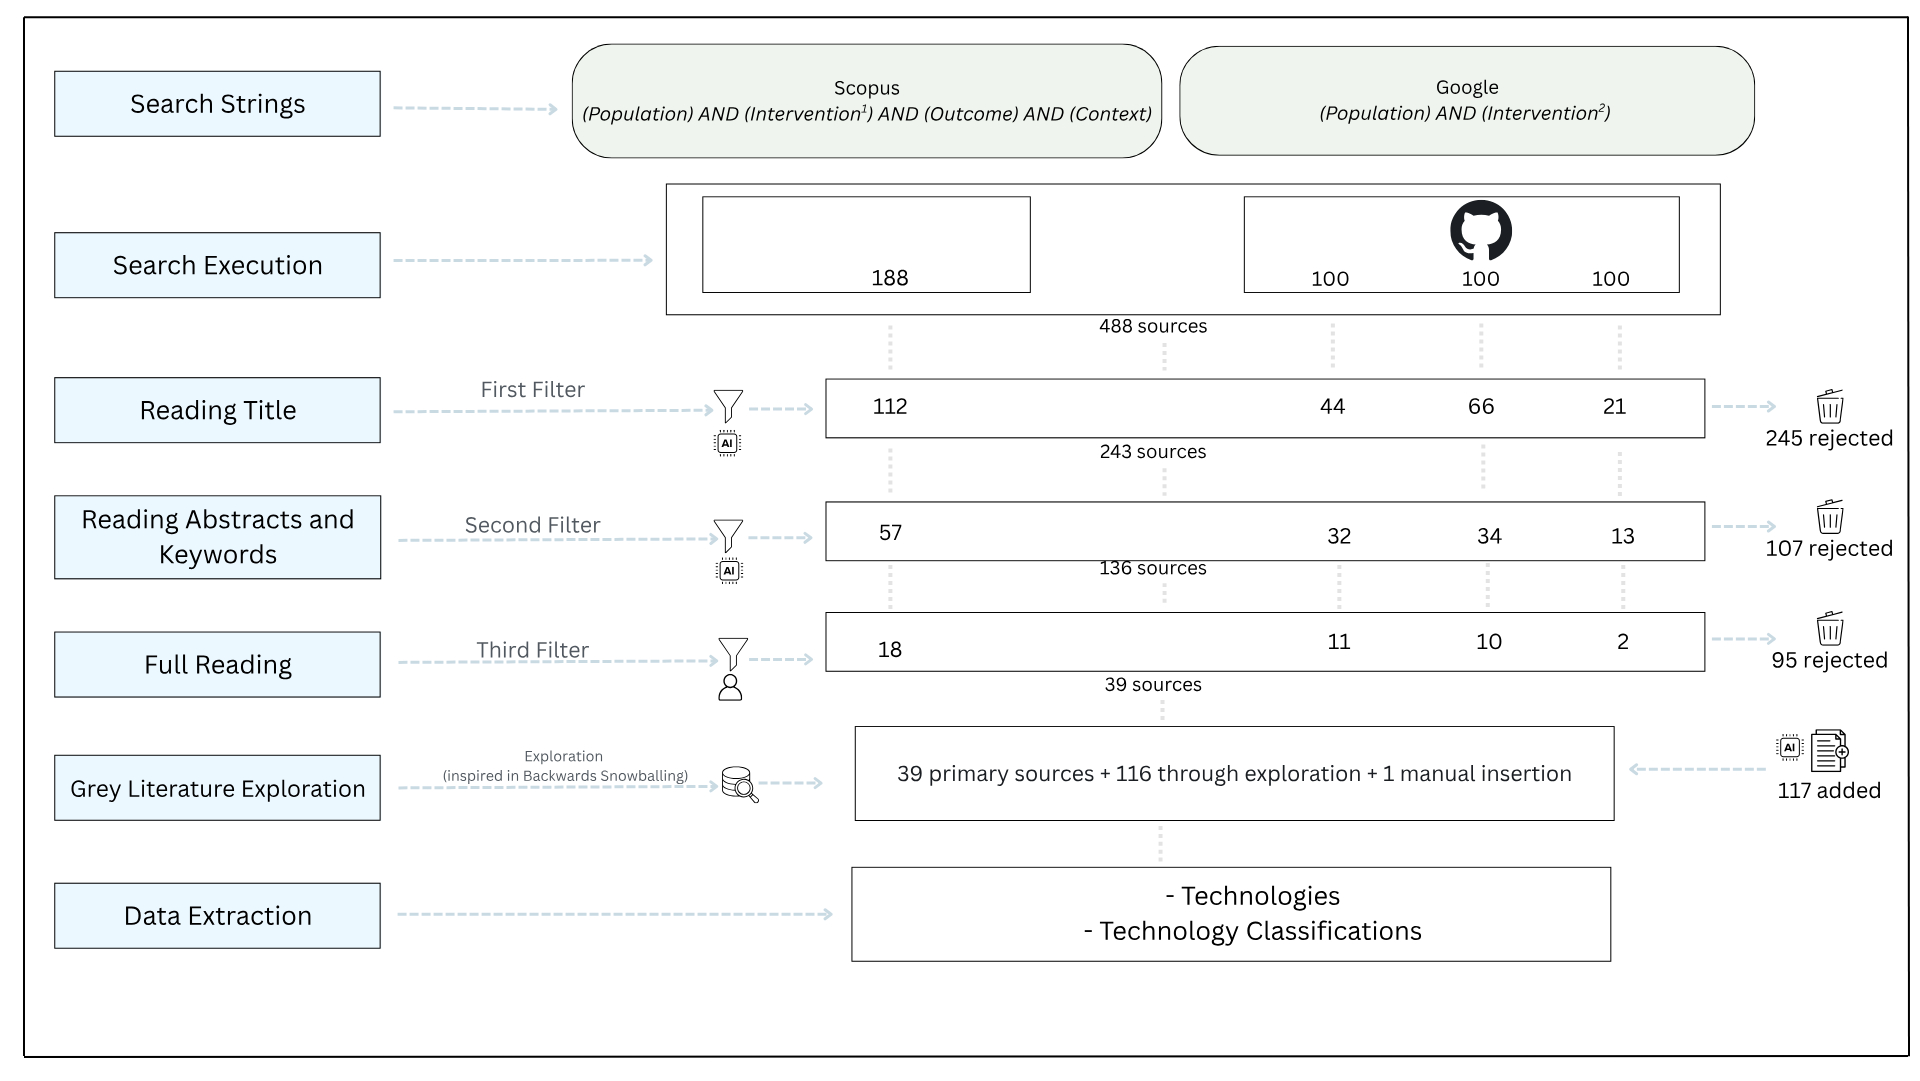
\includegraphics[width=\textwidth]{figures/search-strings.jpg}
    \caption{Methodology used in searching and filtering}
    \label{fig:workflow}
\end{center}
\end{figure*}

